\documentclass[convert]{standalone}

\usepackage{amssymb}
%%%%%%%%%%%%%% Tikz commands %%%%%%%%%%%%%%
\usepackage{tikz}
\usetikzlibrary{positioning}

\makeatletter
\def\absdot{\@ifnextchar[{\@absdotlabel}{\@absdotnolabel}}
	\def\@absdotlabel[#1]#2{%
		\node at #2 {\normalsize \mybullet};
		\node at #2 [below=2pt] {\ensuremath{#1}};
	}
	\def\@absdotnolabel#1{%
		\node at #1 {\normalsize \mybullet};
	}

\def\abssquare{\@ifnextchar[{\@abssquarelabel}{\@abssquarenolabel}}
	\def\@abssquarelabel[#1]#2{%
		\node at #2 {\normalsize \mysquare};
		\node at #2 [below=2pt] {\ensuremath{#1}};
	}
	\def\@abssquarenolabel#1{%
		\node at #1 {\normalsize \mysquare};
	}

\def\abstriangle{\@ifnextchar[{\@abstrianglelabel}{\@abstrianglenolabel}}
	\def\@abstrianglelabel[#1]#2{%
		\node at #2 {\normalsize \mytriangle};
		\node at #2 [below=2pt] {\ensuremath{#1}};
	}
	\def\@abstrianglenolabel#1{%
		\node at #1 {\normalsize \mytriangle};
	}

\makeatother
%%%% Dot %%%%
\newcommand\mybullet{\raisebox{-5pt}{\scalebox{1.5}{\normalsize \ensuremath{\bullet}}}}
\newcommand\mycoloredbullet[1]{\raisebox{-5pt}{\scalebox{1.5}{\normalsize \ensuremath{\color{#1} \bullet}}}}
\newcommand{\absdotcolor}[2]{%
	\node at #1 {\normalsize \mycoloredbullet{#2}};
}
\newcommand{\absdotcolorlabel}[3]{%
	\node at (#1,#2) {\normalsize \mycoloredbullet{#3}};
	\node[label=left:{\color{#3} #2}] at (0.95,#2) {};
}
%%%% Star %%%%
\newcommand\mystar{\raisebox{-5pt}{\normalsize \ensuremath{\bigstar}}}
\newcommand\mycoloredstar[1]{\raisebox{-5pt}{\normalsize \ensuremath{\color{#1} \bigstar}}}
\newcommand{\absstarcolor}[2]{%
	\node at #1 {\normalsize \mycoloredstar{#2}};
}
\newcommand{\absstarcolorlabel}[3]{%
	\node at (#1,#2) {\normalsize \mycoloredstar{#3}};
	\node[label=left:{\color{#3} #2}] at (0.95,#2) {};
}
%%%% Square %%%%
\newcommand\mysquare{\raisebox{-5pt}{\footnotesize \ensuremath{\blacksquare}}}
\newcommand\mycoloredsquare[1]{\raisebox{-5pt}{\normalsize \ensuremath{\color{#1} \blacksquare}}}
\newcommand{\abssquarecolor}[2]{%
	\node at #1 {\normalsize \mycoloredsquare{#2}};
}
\newcommand{\abssquarecolorlabel}[3]{%
	\node at (#1,#2) {\normalsize \mycoloredsquare{#3}};
	\node[label=left:{\color{#3} #2}] at (0.95,#2) {};
}
%%%% Triangle %%%%
\newcommand\mytriangle{\scalebox{1.4}{\raisebox{-5pt}{\normalsize \ensuremath{\blacktriangle}}}}
\newcommand\mycoloredtriangle[1]{\scalebox{1.4}{\raisebox{-5pt}{\normalsize \ensuremath{\color{#1} \blacktriangle}}}}
\newcommand{\abstrianglecolor}[2]{%
	\node at #1 {\normalsize \mycoloredtriangle{#2}};
}
\newcommand{\abstrianglecolorlabel}[3]{%
	\node at (#1,#2) {\normalsize \mycoloredtriangle{#3}};
	\node[label=left:{\color{#3} #2}] at (0.95,#2) {};
}
%%%% Circle %%%%
\newcommand\mycirc{\raisebox{-5pt}{\normalsize \ensuremath{\circ}}}
\newcommand\mycoloredcirc[1]{\raisebox{-5pt}{\normalsize \ensuremath{\color{#1} \circ}}}
\newcommand{\abscirccolor}[2]{%
	\node at #1 {\normalsize \mycoloredcirc{#2}};
}
\newcommand{\abscirccolorlabel}[3]{%
	\node at (#1,#2) {\normalsize \mycoloredcirc{#3}};
	\node[label=left:{\color{#3} #2}] at (0.95,#2) {};
}
%%%% Other %%%%
\newcommand{\colorednumber}[3]{%
	\node at (#1, 0) {\color{#3} #2};
}

\newcommand{\plotperm}[1]{%
	\foreach \j [count=\i] in {#1} {
		\absdot{(\i,\j)};
	};
}

\newcommand{\hook}[5][black]{%
	\draw [draw=#1, very thick] (#2,#3) |- (#4,#5);
}
\usepackage{color}
% \definecolor{lightgray}{rgb}{0.8, 0.8, 0.8}
% \definecolor{darkgray}{rgb}{0.7, 0.7, 0.7}
\definecolor{darkgreen}{rgb}{0,0.5,0}
%%%%%%%%%%%%%%%%%%%%%%%%%%%%%%%%%%%%%%%%%%%

\begin{document}
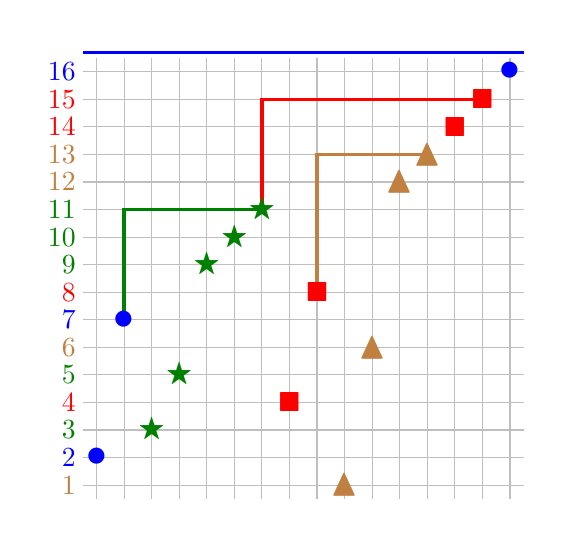
\begin{tikzpicture}[scale=0.35]
	
	% \useasboundingbox (-1,-1) rectangle (18,18);
	% \draw [fill=white, draw=none] (-1.2,-0.1) rectangle (17.2,17.3);
	\draw [fill=white, draw=none] (-1.5,-0.4) rectangle (17.5,17.6);
	\draw [lightgray] (0.5,0.5) grid ++(16,16);
	
	\def\firsthookcolor{blue}
	\def\secondhookcolor{darkgreen}
	\def\thirdhookcolor{red}
	\def\fourthhookcolor{brown}
	
	\hook[\thirdhookcolor]{7}{11}{15}{15}
	\hook[\secondhookcolor]{2}{7}{7}{11}
	%\hook[\firsthookcolor]{0.5}{0.5}{17-0.5}{17-0.5}
	\draw[\firsthookcolor, very thick] (0.5,16.7) --(16.5,16.7);
	\hook[\fourthhookcolor]{9}{8}{13}{13}
	
	\absdotcolorlabel{ 1}{ 2}{\firsthookcolor}
	\absdotcolorlabel{ 2}{ 7}{\firsthookcolor}
	
	\absstarcolorlabel{ 3}{ 3}{\secondhookcolor}
	\absstarcolorlabel{ 4}{ 5}{\secondhookcolor}
	\absstarcolorlabel{ 5}{ 9}{\secondhookcolor}
	\absstarcolorlabel{ 6}{10}{\secondhookcolor}
	\absstarcolorlabel{ 7}{11}{\secondhookcolor}
	
	\abssquarecolorlabel{ 8}{ 4}{\thirdhookcolor}
	\abssquarecolorlabel{ 9}{ 8}{\thirdhookcolor}
	
	\abstrianglecolorlabel{10}{ 1}{\fourthhookcolor}
	\abstrianglecolorlabel{11}{ 6}{\fourthhookcolor}
	\abstrianglecolorlabel{12}{12}{\fourthhookcolor}
	\abstrianglecolorlabel{13}{13}{\fourthhookcolor}
	
	\abssquarecolorlabel{14}{14}{\thirdhookcolor}
	\abssquarecolorlabel{15}{15}{\thirdhookcolor}
	
	\absdotcolorlabel{16}{16}{\firsthookcolor}
%		
%		\foreach \val [count=\idx] in {2,7,3,5,9,10,11,4,8,1,6,12,13,14,15,16} {
%		%	\absdot{(\idx,\val)}
%			\node at (-0.25,\val) {$\val$};
%		}

\end{tikzpicture}
\end{document}  
